%!TEX root = Slic3r-Manual.tex

\subsection{Brim and Raft} % (fold)
\label{sec:brim_and_raft}

\subsubsection{Brim} % (fold)
\label{sub:brim}
\index{brim}

Both simple and expert mode gives the option to add a brim to the first layer of the print.  This is simply additional perimeters around the outside of the model which increases the amount of material holding onto the bed in an effort to reduce warping.  It is also useful for increasing the surface area of small yet tall prints which may otherwise be knocked off the bed mid-print.

Once completed the brim is removed from the print using a sharp utility knife or scalpel.

\begin{figure}[H]
\centering
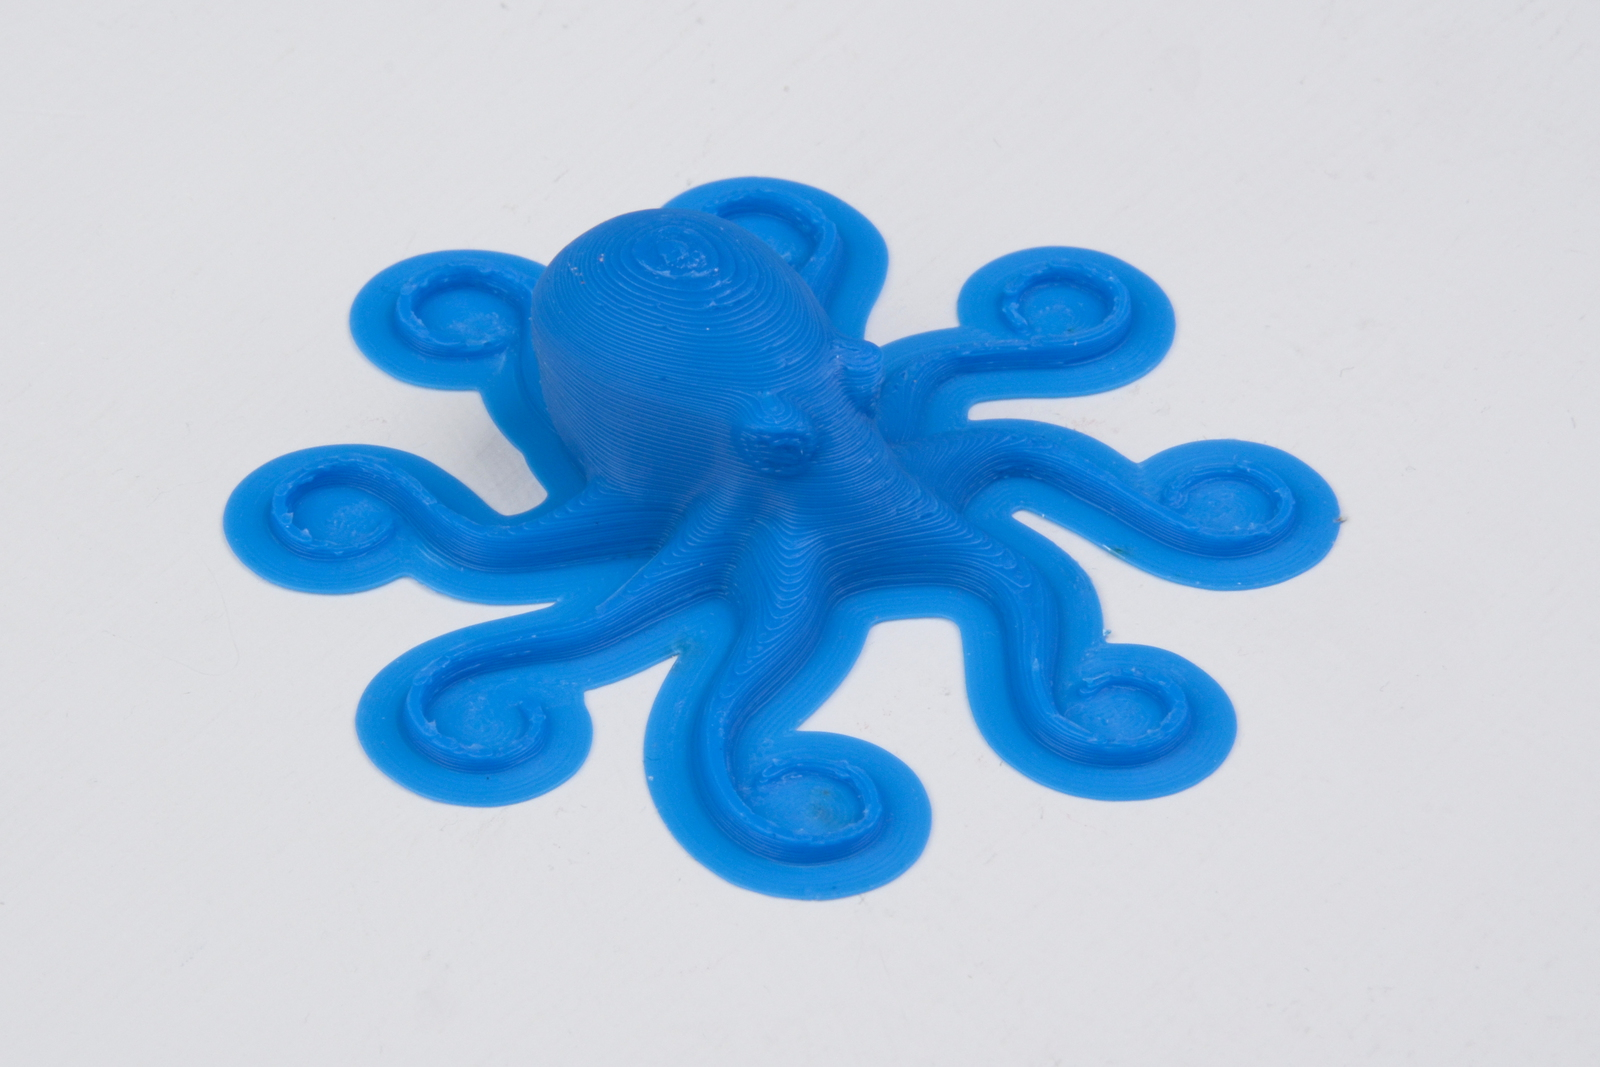
\includegraphics[keepaspectratio=true,width=0.75\textwidth]{tuning/brim.JPG}
\caption{Print with brim.}
\label{fig:print_with_brim}
\end{figure}

% subsection brim (end)

\begin{comment}

\subsubsection{Raft} % (fold)
\label{sub:raft}
\index{raft}

A technique dating back to the early days of 3D printing, a raft is a support structure printed underneath the model.  Because the raft extrusion is usually quite wide it adds more surface area for the print, and additionally covers any surface irregularities in the bed material, should they exist.  The raft technique is particularly popular when printing with ABS as it tends to warp more than PLA.

Again, the raft is expected to be removed manually after the print is completed.

A raft is added by turning on the support option and configuring how many layers should be printed to make up the raft.  As with support structures, the raft is printed rather loosely and the model is not pressed into it too much, in order that it may be easily removed afterwards.

\begin{figure}[H]
\centering

\includegraphics[keepaspectratio=true,width=0.75\textwidth]{placeholder.jpg}
\caption{Print with raft.}
\label{fig:print_with_raft}
\end{figure}

\end{comment}

% subsection raft (end)

% section brim_and_raft (end)
